%%%%%%%%%%%%%%%%%%%%%%%%%%%%%%%%%%%%%%%%%%%%%%%%%%%%%%%%%%%%%%%%%%%%%%%%%%%%%%%%
%2345678901234567890123456789012345678901234567890123456789012345678901234567890
%        1         2         3         4         5         6         7         8

\documentclass[letterpaper, 10 pt, conference]{ieeeconf}  % Comment this line out
                                                          % if you need a4paper
%\documentclass[a4paper, 10pt, conference]{ieeeconf}      % Use this line for a4
                                                          % paper

\IEEEoverridecommandlockouts                              % This command is only
                                                          % needed if you want to
                                                          % use the \thanks command
\overrideIEEEmargins
%\usepackage[czech]{babel}
\usepackage[utf8]{inputenc}
\usepackage{float}
\usepackage{wrapfig}
\usepackage{array}
%\usepackage{sidecap}
% See the \addtolength command later in the file to balance the column lengths
% on the last page of the document



% The following packages can be found on http:\\www.ctan.org
\usepackage{graphicx} % for pdf, bitmapped graphics files
\usepackage{bibentry}
\usepackage{url}
%\usepackage[nottoc]{tocbibind}
%\usepackage{url}
%\usepackage[nottoc]{tocbibind}
\nobibliography*
\usepackage{hyperref}
%\usepackage{epsfig} % for postscript graphics files
%\usepackage{mathptmx} % assumes new font selection scheme installed
%\usepackage{times} % assumes new font selection scheme installed
%\usepackage{amsmath} % assumes amsmath package installed
%\usepackage{amssymb}  % assumes amsmath package installed
\usepackage{listings,multicol} % for code listings, multicolumned
\lstset{% escape sequence inside listing
  escapeinside={(*}{*)},%
}
\usepackage{dtsyntax} % for listings modelica
\usepackage{amsmath} % for mathematical equation
\usepackage{amssymb} % for special symbols - blacktriangledown
\DeclareUnicodeCharacter{00A0}{~}
\title{\LARGE \bf
Experiences in teaching of modeling and simulation with emphasize on equation based and acausal modeling techniques.
}

%\author{ \parbox{3 in}{\centering Tomas Kulhanek*
%         \thanks{*Use the $\backslash$thanks command to put information here}\\
%         Faculty of Electrical Engineering, Mathematics and Computer Science\\
%         University of Twente\\
%         7500 AE Enschede, The Netherlands\\
%         {\tt\small h.kwakernaak@autsubmit.com}}
%         \hspace*{ 0.5 in}
%         \parbox{3 in}{ \centering Pradeep Misra**
%         \thanks{**The footnote marks may be inserted manually}\\
%        Department of Electrical Engineering \\
%         Wright State University\\
%         Dayton, OH 45435, USA\\
%         {\tt\small pmisra@cs.wright.edu}}
%}

\author{\parbox{3 in}{
Tomáš Kulhánek$^{*,1}$, 
Filip Ježek$^{1,2}$, 
Marek Mateják$^{1}$,  
Jan Šilar$^{1}$, 
%Pavol Privitzer$^{1}$, 
%Martin Tribula$^{1}$ 
and Jiří Kofránek$^{1}$}% <-this % stops a space
\thanks{$^{*}$corresponding author {\tt\small tomas.kulhanek@lf1.cuni.cz}}%        
\thanks{$^{1}$Institute of Pathological Physiology, First Faculty of Medicine, Charles University in Prague, Czech Republic}%        
\thanks{$^{2}$Faculty of Electrical Engineering, Czech Technical University in Prague}%
}
\makeatletter
\newcommand*{\inlineequation}[2][]{%
  \begingroup
    % Put \refstepcounter at the beginning, because
    % package `hyperref' sets the anchor here.
    \refstepcounter{equation}%
    \ifx\\#1\\%
    \else
      \label{#1}%
    \fi
    % prevent line breaks inside equation
    \relpenalty=10000 %
    \binoppenalty=10000 %
    \ensuremath{%
      % \displaystyle % larger fractions, ...
      #2%
    }%
    ~\@eqnnum
  \endgroup
}
\makeatother
\begin{document}



\maketitle
\thispagestyle{empty}
\pagestyle{empty}


%%%%%%%%%%%%%%%%%%%%%%%%%%%%%%%%%%%%%%%%%%%%%%%%%%%%%%%%%%%%%%%%%%%%%%%%%%%%%%%%
\begin{abstract}

This work introduces experiences of teaching modeling and simulation in the field of biomedical engineering. We emphasize the acausal and object-oriented modeling technique and we have moved from teaching block-oriented tool MATLAB Simulink to acausal and object oriented Modelica language, which can express the structure of the system rather than a process of computation. 
However, block-oriented approach is allowed in Modelica language too and students have tendency to express the process of computation. Usage of the exemplar acausal domains and approach allows students to understand the modeled problems much deeper. The causality of the computation is derived automatically by the simulation tool.
\end{abstract}


%%%%%%%%%%%%%%%%%%%%%%%%%%%%%%%%%%%%%%%%%%%%%%%%%%%%%%%%%%%%%%%%%%%%%%%%%%%%%%%%
\section{Introduction}
An important aspect of biomedical engineering is the ability to mathematically formalize the scientific knowledge in biomedicine and utilize such formalization -- model -- in engineering use cases like simulation, prediction, decision support etc. 

There are several approaches, how a mathematical model can be expressed and implemented in an execution code which can be simulated using computers. One approach is to directly incorporate mathematical equations of the model as statements in some programming language code. This includes process of (1) definition of system, (2) decomposition of the system to subsystems, (3) modeling of the subsystems, (4) derivation of the computation causality and (5) implementation in programming language.
Another approach is to separate the mathematical model from it's simulator code and allow expressing the causality of the computation model in some higher level programming language and reduce the time of implementation (5). Such tools are usually denoted as block oriented languages. Examples are, e.g., industrial tool MATLAB Simulink, or domain specific languages to model physiology JSIM (NSR Physiome project introduced a JSIM Java based simulation system to support modeling in  physiology and introduces a repository of several hundred of models \cite{Butterworth2014}), CellML (IUPS Physiome project introduced XML based standard CellML and FieldML, tools and repository \cite{Hunter2004,Yu2011}), SBML (Systems Biology Markup Language (SBML) is used for modeling biological system at the level of biochemical reaction and regulatory network \cite{Hucka2004}).

One of the first complex model of integrative physiology was model of circulatory system with it's control regulation published by Guyton et al. \cite{Guyton1972}. This model was originally implemented in generic programming language FORTRAN and it gradually evolved to the current model HumMod published by Hester et al. \cite{Hester2011systems,hester2011}. It is not implemented in some programming language directly, they rather use an in-house XML-based domain specific language and tool to interpret and solve this model. Kofránek and Rusz published implementation of the Guyton's original model in MATLAB Simulink \cite{Kofranek2010}. Due to the complexity of further integrative models, it becomes harder to maintain and keep the complex model updated and flexible using the mentioned modeling technology and tools. One of the reason is that the model express the process of computation.  
Therefore, Kofránek et al. chose acausal and object-oriented modeling language Modelica and implemented the current HumMod model in the standardized Modelica language \cite{Kofranek2011hummod}. Recently we have shown that the block oriented aproach in modeling pulsatile cardiovascular system introduced by Fernandez de Canete et al.\cite{FernandezdeCanete2014} may bring problems of further development and understandability. An acausal approach was shown by Kulhánek et al.\cite{Kulhanek2014Modeling}.

%The acausal modeling technique seems to be one of the key features to maintain complex models as the model diagrams still captures the essence of the modeled reality much better and the simulation models are much more legible and thus less prone to mistakes \cite{Kofranek2008,FernandezDeCanete2013}.

Because no other modeling technology was suitable for the complex model Hummod, we started to teach the Modelica language within the classes of modeling and simulation which is executed within the last year of biomedical engineering curriculum with preliminary results promising good acceptance published by Ježek et al.\cite{Jezek2012}.
Additionally, educational text in czech language was published by Kofránek et al.\cite{kofranek2013Pacientske} to support the courses of biomedical engineering with focus on patient simulator and modeling methodology with an example of modeling cardiovascular system published originally by Meurs \cite{Meurs2011} and used in the \textregistered Human Patient Simulator produced by CAE HealthCare\footnote{\url{http://www.caehealthcare.com/} accessed April 2015}. Such models and simulators are used further in teaching of students of medicine. This  education methods and tools are shared within MEFANET network, Czech and Slovak Medical Faculties Network \cite{Schwarz2014}.

The students of biomedical engineering (of Czech Technical University in Prague, Czech Republic) are familiar with generic programming languages like C++, Java or interpreted Python etc. They are familiar with block-oriented modeling and simulation techniques and capabilities of MATLAB Simulink. 
%And when faced up with the task to express mathematical model published in scientific paper they usually use a block-oriented (causal) approach which leads to the implementation of process of computation. Although, this approach is possible also in Modelica language, we concluded that using acausal approach with  object-oriented techniques can lead to more understandable and maintainable models describing more complex systems.

This work summarizes the main methods of acausal modeling technique in connection with some selected physiological or physical phenomenon. The results is based on the semestral work which is done by students at the end of the course, which shows their ability to cover medium complex phenomenon in integrative way which is essential for further work with complex models incorporating current state-of-the-art knowledge about modeled system.

%This block-oriented modeling technique lead to describing the process of computation, which has a benefit of full control on the computation process without the need to do such stuff in some generic programming languages like C++, FORTRAN etc.


%One approach is to standardize the academic grown tools and language to describe physiological system. E.g. the NSR Physiome project introduced a JSIM Java based simulation system to support modeling in  physiology and introduces a repository of several hundred of models\cite{Butterworth2014,jsim}. The similar effort is done by IUPS Physiome project and it's XML based standard CellML and FieldML, where tools and repository of models are presented \cite{Hunter2004,Yu2011}. The Systems Biology Markup Language (SBML) is used for modeling biological system at the level of biochemical reaction and regulatory network\cite{Hucka2004}. JSIM, CellML, SBML or HumMod are domain specific language and the tools and environment are primarily developed to model physiology or systems biology. 

%Another approach is to use commercial or industry standard tools for mathematical modeling e.g. %Fernandez de Canete et al. described a closed loop cardiovascular model and mechanism of arterial pressure control in MATLAB\textsuperscript{\textregistered} based modeling module SIMSCAPE\texttrademark\cite{FernandezDeCanete2013} and recently in Modelica language and DYMOLA tool\cite{FernandezDeCanete2014}. 




%For the complex models this seems to bring disadvantages for more complex phenomenon or integrative approach. 

 
%Hester et al. published HumMod - a large scale physiological model, constructed from empirical data obtained from peer-reviewed physiological literature \cite{hester2011}. Kofranek et al. translated and maintain HumMod-Golem Edition model in the standardized Modelica language which may be more understandable \cite{Kofranek2011hummod}. Modelica \cite{Modelica} tools offer simulation environment or the model can be exported into a package conforming standard FMI and integrated into custom application. 

\section{Methods}

%Acausal modelica, library for acausal modeling of physiology - physiolibrary.
%Different domains similar principles.

Modelica language maintained by the Modelica association is object oriented, equation based and acausal modeling language (\url{http://www.modelica.org}). A Modelica model can be presented by its icon (the icon is used in further model diagrams), defined with a textual notation (source code listing in further text) or defined by diagrams (figures in further text). We recommend textual form to express equations of basic subsystem describing domain specific laws and diagram form to express composition of several basic components. Further reading about Modelica is in published works of Fritzson \cite{fritzson2010} or free accessible online book of Tiller\cite{Tiller2014}.

\emph{Object orientation} means that model is defined as a class, which can be instantiated. Each instance share type and differ in parameters and the place where it is used. Inheritance and some sort of polymorphism is possible. \emph{Equation based} means that the model can be expressed using equations instead of assignment statements. Modelica tool will decide which variable is input and output upon compilation. \emph{Acausal} means that the model composed of several submodel do not need explicitly declare what is input and output. Acausal connector is special purpose class to define variables of the model shared with other models or classes. Connecting two or more components via acausal connector will generate analogy of Kirchhoff's law equations, which ensure equality of all "non-flow" variables in connectors \inlineequation[eq:kirchhoff1]{p_1=p_2=\ldots =p_n} 
and zero sum of all "flow" variables \inlineequation[eq:kirchhoff2]{\sum_{i=1}^n q_i=0}

The basics of various systems can be explained using analogy between domains. Not only electrical and mechanical domains are analogous \cite{firestone1933}. Analogies exist among hydraulic, thermodynamic and chemical domain too \cite{kofranek2013Pacientske}.

We use the following domains and examples to show the analogies among different domains with focus on acausal and object oriented approach. 

\subsection{Hydraulic domain}

Hydraulic domain can be used to express cardiovascular system (CVS) using Windkessel approach\cite{Kulhanek2014mefanet}. CVS can be decomposed into abstract component expressing hydraulic elasticity and hydraulic resistance. Connector \emph{HydraulicPort} with "flow" variable $q$ and non-flow variable pressure $p$ is presented by it's Icon and by the Modelica source code definition:

\begin{tabular}{cl}
Icon & Modelica source \\
\hline

\includegraphics[width=0.03\textwidth]{Connector.png} & \begin{lstlisting}[language=modelica, backgroundcolor=\color{white}] 
connector HydraulicPort  
  flow Real q; 
  Real p; 
end HydraulicPort;  
\end{lstlisting}\\

\end{tabular}

Model of hydraulic resistor(conductor) with parameter $G$ denoting conductance and two hydraulic ports is expressed by the equations:
\begin{equation}
q_{in}.q = -q_{out}.q \label{eq:conductor1}
\end{equation} 
\begin{equation}
 q_{in}.q = G \times (q_{in}.p-q_{out}.p) \label{eq:conductor2}
\end{equation}
Model of hydraulic elastance, with parameters $V_0$ as unstressed volume, $p_0$ external pressure and $C$ compliance(reciprocal value of elastance) with state variable $V$ volume, is expressed by these equations:
\begin{equation} \label{eq:elastic1}p-p_0 = \left\{   
  \begin{array}{l l} 0 & \quad \text{if } V \text{\textless} V_0 \\ 
    \frac{V-V_0}{C} & \quad \text{otherwise}
  \end{array} \right.\end{equation} 
\begin{equation}\label{eq:elastic2}\frac{{\rm d}V}{{\rm d}t} =  q\end{equation} 
Both models can be written in Modelica.

\begin{tabular}{cl}
Icon & Modelica source \\
\hline
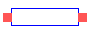
\includegraphics[width=0.03\textwidth]{Resistance.png} & 
\begin{lstlisting}[language=modelica, backgroundcolor=\color{white}]
model HydraulicConductor
  parameter Real G;
  HydraulicPort qin;
  HydraulicPort qout;
equation 
  qin.q= -qout.q; // eq.(3)
  qin.q = G*(qin.p-qout.p); // eq.(4)
end HydraulicConductor;
\end{lstlisting} \\
\hline

\includegraphics[width=0.03\textwidth]{Elasticity.png} & 
\begin{lstlisting}[language=modelica, backgroundcolor=\color{white}]
model HydraulicElastance
    Real V;
    parameter Real V0;
    parameter Real p0;
    parameter Real C;
    HydraulicPort qin;
equation 
   // eq.(5)
  qin.p-p0 = if (V<V0) then 0 else (V-V0)/C;
  der(V) = qin.q; // eq.(6)
end HydraulicElastance;
\end{lstlisting}
\end{tabular}

This can be used to model two ideal baloons with liquid  interconnected via a tube characterized by some resistance. The acausal connectors \emph{qin} and \emph{qout} are connected via the \emph{connect()} statement in the following listing:
\begin{lstlisting}[language=modelica]
model twoballons
  HydraulicConductor systemicResistance;
  HydraulicElastance arteries;
  HydraulicElastance veins;
equation 
  connect(arteries.qin, systemicResistance.qin);
  connect(systemicResistance.qout, veins.qin);
end twoballons;
\end{lstlisting}

This textual form is equivalent to the diagram form in Figure \ref{fig:twoballons}.
\begin{figure}[h!]
    \centering
    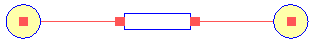
\includegraphics[width=0.4\textwidth]{twoballons.png}
    \caption{Diagram, which connects two HydraulicElastance and HydraulicResistance represented by its icons via acausal connectors. Each connection (blue line between blue squares) generates the Modelica "connect" statement above.
    }
    \label{fig:twoballons}
\end{figure}

The concrete instances may differ according to what is known about the system, either by external measurement, or by some superior model. The \emph{ballsVolume} is initialized with initial volume of first balloon $V(start) = 5000$ and by setting parameter values of $V_0$, $p_0$, $C$ and $G$ as seen in the following Modelica listing:

\begin{lstlisting}[language=modelica]
model ballsVolume
  extends twoballons(
    arteries(
      V(start=5000),
      V0=529,
      p0=0,
      C=1.5),
    systemicResistance(G=1),
    veins(
      V0=2845,
      p0=0,
      C=200));
end ballsVolume;
\end{lstlisting}

The Modelica tool will decide automatically which variables will be dependent and which independent. Computation flow is solved as seen from the following generated code (note the assignment statement \emph{:=}).
\begin{lstlisting}[language=modelica]
// Translated M. model generated by Dymola  
//  ballsVolume
...
// Dynamics Section
  systemicResistance.qout.p := veins.p0+
    (if veins.V < veins.V0 then 0 
    else (veins.V-veins.V0)/veins.C);
  systemicResistance.qin.p := arteries.p0+
    (if arteries.V < arteries.V0 then 0
    else (arteries.V-arteries.V0)/arteries.C);
  der(arteries.V) := systemicResistance.G*
    (systemicResistance.qout.p-
      systemicResistance.qin.p);
  der(veins.V) :=  -der(arteries.V);
\end{lstlisting}

When simulated the system goes to some equilibrium, steady state, which illustrates  that the liquid has tendency to go from the compartment with higher pressure to compartment with lower pressure until the pressures are ballanced. In physiology, the blood has tendency to flow from arteries (having low compliance) to veins (having high compliance).

%It is possible to add additional components to model hydraulic valve, inertia, etc. Matejak et al. published the Modelica library containing the hydraulic domain and additional components for chemical domain, osmotic and thermal domain, which are useful for buidling complex models of human physiology not only in the textual form introduced above, but also using graphical diagrams \cite{Matejak2014,Matejak2014mj}.  
\subsection{Spring/Mass System}

An example of harmonic oscillator is decomposed into mass, fix, spring and joint subsystems. 
The mass is characterized by the parameter $m$ and following equations among $F$--force, $a$--acceleration:
\begin{equation}
F = m \times a \label{eq:fma}
\end{equation} 
\begin{equation}
a = \frac{\mathrm{d}^2 y}{\mathrm{d}t^2} \label{eq:ady}
\end{equation}

The spring is characterized by the parameter $k$--stiffness and following equations among $F$--force, $dy$--displacement:
\inlineequation[eq:f1f2]{F_1 = F_2}
\inlineequation[eq:fkdy]{F = -k\times dy}
\inlineequation[eq:fma2]{F = m \times a}
\inlineequation[eq:dy2y1]{dy = y_2-y_1}

The fixed point is characterized by the fixed position set to 0:
\inlineequation[eq:y0]{y = 0}

The joint is presented as acausal connector similar way as in the hydraulic domain. But contrary to common understanding, $F$--force is the "flow" variable and $y$--position is "non-flow" variable. The Modelica implementation of these subsystem is in Modelica listing in Table \ref{spring}.
\begin{table}
\begin{tabular}{cl}
Icon & Modelica source \\
\hline
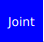
\includegraphics[width=0.03\textwidth]{joint.png} & 
\begin{lstlisting}[language=modelica, backgroundcolor=\color{white}]
connector MechanicalJoint
  Real y "position";
  flow Real F "force";
end MechanicalJoint;
\end{lstlisting} \\
\hline

\includegraphics[width=0.03\textwidth]{fix.png} & 
\begin{lstlisting}[language=modelica, backgroundcolor=\color{white}]
model MechanicalFix
  MechanicalJoint mechanicalJoint;
equation 
  mechanicalJoint.y=0;
end MechanicalFix;
\end{lstlisting}\\
\hline
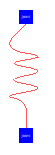
\includegraphics[width=0.03\textwidth]{spring.png} & 
\begin{lstlisting}[language=modelica, backgroundcolor=\color{white}]
model MechanicalSpring
  Real dy "displacement";
  parameter Real k= 10;
  MechanicalJoint upperJoint;
  MechanicalJoint lowerJoint;
equation 
   lowerJoint.F = -k * dy;
   upperJoint.F +lowerJoint.F = 0;
   dy = upperJoint.y - lowerJoint.y;
end MechanicalSpring;
\end{lstlisting}\\
\hline
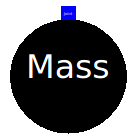
\includegraphics[width=0.03\textwidth]{mass.png} & 
\begin{lstlisting}[language=modelica, backgroundcolor=\color{white}]
model MechanicalMass
  MechanicalJoint mechanicalJoint;
  Real y "position of the mass";
  parameter Real initPos=0 "initial position";
  parameter Real m "mass";
  Real a "acceleration";
  Real v "velocity";
initial equation 
  y=initPos;
equation 
  mechanicalJoint.y = y;
  mechanicalJoint.F = m * a;
  v = der(y);
  a = der(v);
end MechanicalMass; 
\end{lstlisting}
\end{tabular}
\caption{Spring/Mass system components in Modelica.}
\label{spring}
\end{table}

This can be used to model two springs connected serially e.g. as a diagram view in Figure \ref{fig:twosprings}. 

\begin{wrapfigure}{l}{0.1\textwidth}
  \begin{center}
    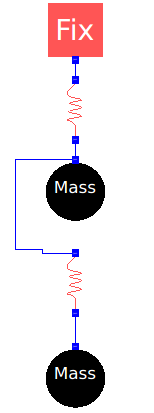
\includegraphics[width=0.1\textwidth]{twosprings.png}
  \end{center}
  \caption{Springs}
  \label{fig:twosprings}
\end{wrapfigure}


Diagram of two springs connects fixed point with first spring with a mass and second spring with another mass is connected to the first spring. If such system  will be solved using the equations (\ref{eq:fma})..(\ref{eq:y0}) then the following set of differential equations need to be solved:


\begin{equation}
m_1\frac{\mathrm{d}^2 y_1}{\mathrm{d}t^2}-k_2(y_2-y_1)+k_1y1 = 0
\label{eq:s1}
\end{equation}
\begin{equation}
m_2\frac{\mathrm{d}^2 y_2}{\mathrm{d}t^2}+k_2(y_2-y_1) = 0
\label{eq:s2}
\end{equation}

Comparison of the equations \ref{eq:s1} and \ref{eq:s2} with the model in Modelica diagram in Figure \ref{fig:twosprings} is used to motivate students in order to decompose system to basic components and use diagrams with appropriate acausal connectors to compose complex system. 
%\addtolength{\textheight}{1cm}   % This command serves to balance the column lengths
                                  % on the last page of the document manually. It shortens
                                  % the textheight of the last page by a suitable amount.
                                  % This command does not take effect until the next page
                                  % so it should come on the page before the last. Make
                                  % sure that you do not shorten the textheight too much.

\subsection{Tools and Libraries}
There are several tools supporting Modelica, we use the commercial Dymola tool (\url{www.dynasim.se}), Wolfram System Modeler (\url{https://www.wolfram.com/system-modeler/}) and open source OpenModelica (\url{https://www.openmodelica.org/}).
Matejak et al. published the Modelica library containing the hydraulic domain and additional components for chemical domain, osmotic and thermal domain, which are useful for building complex models of human physiology \cite{Matejak2014,Matejak2014mj}. We encourage to use this library and other numerous Modelica libraries. 
\subsection{Semester Project}

We provide one-semestral course, enough to show basic concepts of Modelica only. In the end of the course though, the students are capable of implementing a model from biomedical domain on their own. The objective of semester project is to utilize  the taught Modelica language to formalize arbitrary object from biomedical field. Because we emphasize using acausal approach, we force them to use knowledge from neighboring fields (such as physiology, physics, chemistry or biology) and better understand the modeled reality.

%The main competences in modeling and simulation are the abilities to abstract the system, formalize it and interpret the results. While the abstraction and interpretation is merely an art with complex theory, the formalization is mostly a cook-book, provided full model understanding.  When we have formalized model in some of modeling formalization schemes (i.e. modeling or programming language), we are able to execute automatic inference (i.e. simulation) to obtain results data (time-course or steady state model values).

%
%Empirically derived function of flow rate per time going out from the heart:
%\begin{equation} \label{eq:heart} q = \left\{   
%  \begin{array}{l l} 0 & \quad \text{otherwise} \\ 
%    \sin \left( 
%    \frac{t_c-T_{D1} }{ T_{D2} -T_{D1} } * \pi \right) * Q_{peak} 
%    & \quad \text{if } t_c \in (T_{D1}..T_{D2})
%  \end{array} \right.\end{equation} 
%\begin{equation}\label{eq:flowrate2}\frac{{\rm d}V}{{\rm d}t} =  q\end{equation} 
%
%\begin{lstlisting}[language=modelica]
%model HeartFlow
%  HydraulicPort qout;
%  discrete Real T0, HP=0.8;
%  Boolean b(start = false);
%  parameter Real TD1 = 0.07, TD2=0.39, QP = 0.000424;
%  Real tc "relative time in cardiac cycle";
%equation
%  b = time - pre(T0) >= pre(HP) "true if new cardiac cycle begins";
%  when {initial(), b} then
%    T0 = time "set begining of cardiac cycle";
%  end when;
%  tc = time - T0 "relative time in carciac cycle";
%  qout.q=if tc>TD1 and tc<TD2 then sin((tc-TD1)/(TD2-TD1)*Modelica.Constants.pi)*QP else 0;
%end HeartFlow;
%\end{lstlisting}


%%%%%%%%%%%%%%%%%%%%%%%%%%%%%%%%%%%%%%%%%%%%%%%%%%%%%%%%%%%%%%%%%%%%%%%%%%%%%%%%

\section{Results}
The models implemented by students varied from model of small water power plant to model of scooba diver and formation of gas bubbles to model of vocal tract, capable of producing understandable vowel waveforms (\url{http://modelica.creativeconnections.cz/student-works/2014/}). Some students chose to not only implement, but design the model of their own or combine existing models and enhance them, which shows deep understanding of the issue. We state, that when using traditional causal tools, this might not be possible or at least as common. Some students continue and e.g. Dolezalova published demonstration of extracorporeal membrane oxygenation (ECMO)\cite{dolezalova2014}.

Students often use primary literature, where the accompanying models (if present), are most usually either in imperative programming language or block modeling language. Often the first reaction is to hold the block scheme, which is possible in Modelica, but not appropriate for the task, as it does not require deep insight. %However, if a project needs to add or integrate substantial knowledge, the deep insight become essential and acausal approach facilitates it.

%%%%%%%%%%%%%%%%%%%%%%%%%%%%%%%%%%%%%%%%%%%%%%%%%%%%%%%%%%%%%%%%%%%%%%%%%%%%%%%%



%%%%%%%%%%%%%%%%%%%%%%%%%%%%%%%%%%%%%%%%%%%%%%%%%%%%%%%%%%%%%%%%%%%%%%%%%%%%%%%%

\section{Conclusion}

Our students are generally used to choose the easier way, which means to mirror the proposed procedure, without profound understanding. Using acausal approach we make them to really understand the process. Our experience proves, that using acausal modeling deepens the understanding of the model instead of imitate the function only. Using acausal approach, by the end of the course students are capable of creating complex systems with tens to hundreds of equations and still being able to comprehend it as a whole. 


%\section*{ACKNOWLEDGMENT}

\bibliographystyle{unsrturl}
\bibliography{/home/tomaton/Documents/Studium-Dokumenty/Dizertace/bibliography/Dizertace}

\end{document}
